% --- FILE: section/4.system/4.1_architecture_overview.tex ---

\section{Tổng quan kiến trúc hệ thống}
\label{sec:architecture_overview}

\subsection{Mô hình kiến trúc tổng thể}
Hệ thống được thiết kế theo mô hình đường ống (\textit{Pipeline Architecture}), chia thành các mô-đun xử lý tuần tự nhằm giải quyết bài toán truy xuất thông tin từ dữ liệu âm thanh hội họp phức tạp. Mục tiêu thiết kế là đảm bảo khả năng xử lý các cuộc họp kéo dài, đa người nói và cung cấp câu trả lời có độ chính xác cao dựa trên ngữ cảnh thực tế.

Kiến trúc tổng thể của hệ thống bao gồm hai mô-đun chính hoạt động liên kết chặt chẽ:
\begin{enumerate}
    \item \textbf{Mô-đun Xử lý tiếng nói (Speech Processing Module):} Chịu trách nhiệm chuyển đổi dữ liệu âm thanh thô thành văn bản có cấu trúc, bao gồm việc định danh người nói (\textit{Speaker Diarization}) và nhận dạng nội dung (\textit{ASR}).
    \item \textbf{Mô-đun Truy xuất và Tạo sinh tri thức (RAG Module):} Thực hiện việc lưu trữ, đánh chỉ mục vector và sử dụng mô hình ngôn ngữ lớn (\textit{LLM}) để trả lời câu hỏi dựa trên văn bản đã được trích xuất.
\end{enumerate}

Sự tách biệt giữa hai mô-đun này giúp hệ thống đạt được tính độc lập cao, dễ dàng nâng cấp từng thành phần (ví dụ: thay đổi model ASR hoặc model Embedding) mà không ảnh hưởng đến toàn bộ cấu trúc.

% \begin{figure}[h]
%     \centering
%     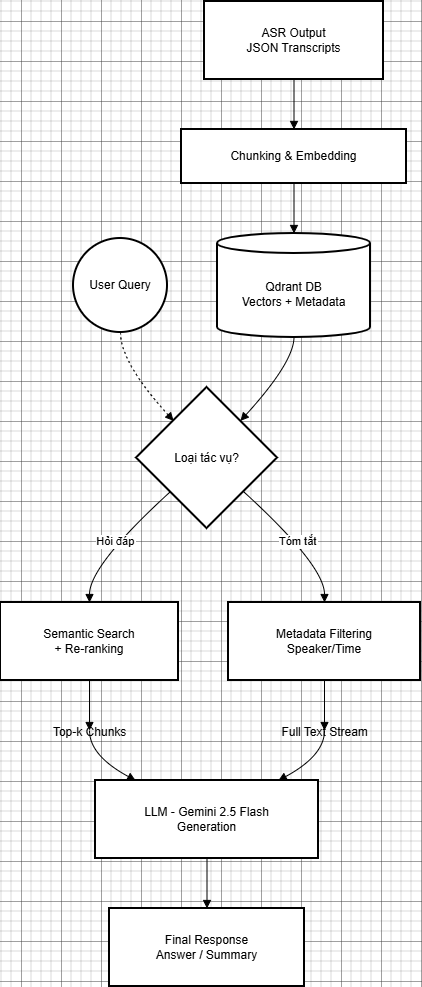
\includegraphics[width=0.9\textwidth]{images/RAG_pipline.png}
%     \caption{Sơ đồ kiến trúc tổng thể của hệ thống hỗ trợ cuộc họp thông minh}
%     \label{fig:system_overview}
% \end{figure}

\subsection{Luồng dữ liệu trong hệ thống}
Dữ liệu trong hệ thống được luân chuyển và biến đổi qua 4 giai đoạn chính, đảm bảo tính vẹn toàn từ tín hiệu âm thanh đến câu trả lời cuối cùng:

\begin{itemize}
    \item \textbf{Giai đoạn 1: Thu thập và Tiền xử lý (Ingestion).} Đầu vào là các bản ghi âm cuộc họp (Meeting Recordings). Các bản ghi này thường chứa tạp âm và có nhiều người tham gia. Hệ thống thực hiện chuẩn hóa âm thanh để tối ưu cho bước nhận dạng.
    
    \item \textbf{Giai đoạn 2: Chuyển đổi cấu trúc (Transcribing \& Diarization).} Phân hệ ASR xử lý tín hiệu âm thanh để tách biệt các đoạn thoại của từng diễn giả và chuyển đổi thành văn bản. Kết quả đầu ra không chỉ là chuỗi ký tự đơn thuần mà là dữ liệu bán cấu trúc (\textit{Semi-structured Data}) chứa thông tin siêu dữ liệu (\textit{Metadata}) quan trọng: định danh người nói (\textit{Speaker ID}) và mốc thời gian (\textit{Timestamp}).
    
    \item \textbf{Giai đoạn 3: Đánh chỉ mục tri thức (Indexing).} Dữ liệu văn bản kèm metadata được phân hệ RAG tiếp nhận. Tại đây, kỹ thuật \textit{Chunking} thông minh được áp dụng để chia nhỏ hội thoại nhưng vẫn giữ nguyên ngữ cảnh. Các đoạn văn bản này sau đó được mã hóa thành vector (\textit{Embeddings}) và lưu trữ trong Cơ sở dữ liệu Vector để phục vụ truy vấn.
    
    \item \textbf{Giai đoạn 4: Truy xuất và Tổng hợp (Retrieval \& Generation).} Khi người dùng đặt câu hỏi (ví dụ: ``Ai đề xuất phương án A?''), hệ thống thực hiện tìm kiếm ngữ nghĩa (\textit{Semantic Search}) kết hợp xếp hạng lại (\textit{Re-ranking}). Các đoạn hội thoại liên quan nhất được trích xuất và đưa vào LLM để sinh câu trả lời, kèm theo dẫn chứng cụ thể về thời gian và người nói.
\end{itemize}

\subsection{Các nguyên lý thiết kế cốt lõi}
Dựa trên đặc thù của bài toán xử lý biên bản cuộc họp, hệ thống tuân thủ các nguyên tắc thiết kế sau:

\begin{enumerate}
    \item \textbf{Tính truy vết (Traceability):} Mọi thông tin do LLM sinh ra đều phải được neo giữ (\textit{grounded}) vào dữ liệu gốc. Hệ thống được thiết kế để luôn trả về nguồn gốc của thông tin (trích đoạn âm thanh tại giây thứ bao nhiêu, do ai nói) để người dùng có thể đối chiếu, đặc biệt quan trọng trong các lĩnh vực pháp lý và y tế.
    \item \textbf{Khả năng chống nhiễu (Robustness):} Nhận thức được việc transcript từ ASR có thể chứa sai sót nhận dạng, cơ chế tìm kiếm Vector được tối ưu hóa để nắm bắt ý nghĩa ngữ nghĩa tổng quát thay vì chỉ so khớp từ khóa chính xác, giúp hệ thống vẫn tìm được thông tin đúng ngay cả khi văn bản có lỗi sai chính tả nhỏ.
    \item \textbf{Xử lý ngữ cảnh dài (Long-context Handling):} Với các cuộc họp kéo dài hàng giờ, hệ thống sử dụng chiến lược cửa sổ trượt (\textit{sliding window}) và bộ nhớ đệm hội thoại để đảm bảo LLM không bị mất ngữ cảnh khi xử lý các câu hỏi phức tạp hoặc các yêu cầu tóm tắt đa tầng (\textit{multi-level summarization}).
\end{enumerate}